\documentclass[11pt, english, fleqn, DIV=15, headinclude, BCOR=2cm]{scrreprt}

\usepackage[
    color,
    bibatend,
]{../../header}

\graphicspath{{./}{../Figures/}}

\usepackage{needspace}

\hypersetup{
    pdftitle=
}

\newcommand\mot{\textsc{mot}}

\usepackage{longtable}
\usepackage{subcaption}

\usepackage[all]{nowidow}

\DeclareMathOperator\sinc{sinc}

\subject{Lab report}
\title{Optical frequency doubling}
\subtitle{Experiment A245 -- Universität Bonn}
\author{%
    Martin Ueding \\
    \small{\href{mailto:mu@martin-ueding.de}{mu@martin-ueding.de}}
    \and
    Lino Lemmer \\
    \small{\href{mailto:l2@uni-bonn.de}{l2@uni-bonn.de}}
}

\date{\daterange{2016-05-23}{2016-05-24}}

\publishers{Tutor: Gautam Ramola}

\begin{document}

\maketitle

\begin{abstract}
    We classify a \SI{987}{\nano\meter} class 3B diode laser and then use it to
    double the frequency within a $\mathrm{KNbO_3}$ crystal. Fundamental wave
    power is measured depending on the crystal temperature, harmonic wave power
    and polarization. The exactness of the doubling is confirmed with a grating
    and a Michelson interferometer.
\end{abstract}

\tableofcontents

\chapter*{Permission to upload}

I, Martin Ueding, would like to scan and upload this lab report with your
corrections to my website \href{http://martin-ueding.de}{martin-ueding.de}.
There, the original lab report as well as the reviewed one will be licensed
under the “\href{http://creativecommons.org/licenses/by-sa/4.0/}{Creative
Commons Attribution-ShareAlike 4.0 International License}”. Is that okay with
you?

Yes $\Box$ \hspace{2cm} No $\Box$

\chapter{Theory}

% \section{Nonlinear optics}
% 
% Light propagating through matter induces a periodic displacement of the
% material's charge carriers, the valence electrons. This leads to a polarization
% $P$ inside the material, which can be expressed as power series in $E$:
% \[
%     P(t) = \epsilon \del{\chi^{(1)}E(t) + \chi^{(2)}E^2(t) + \dots} \, ,
% \]
% where $\epsilon$ is the permittivity and $\chi^{(i)}$ the susceptibility of
% $i$-th order, which in general is a tensor of higher order. The first term is the well known linear polarization which holds for small
% intensities. For higher intensities the nonlinear terms become important.
% 
% \subsection{Second harmonic generation}
% 
% For an incoming plane wave $E = E_0 \sin(\omega t)$ the polarization up to the
% second order can be expressed as
% \[
%     P(t) = \epsilon\del{\chi^{(1)}E_0\sin(\omega t)  + \half\chi^{(2)}E_0^2 
%     - \half\chi^{(2)}E_0^2\cos(2\omega t)} \, .
% \]
% Compared with linear optic two extra terms occur. The first term gives a
% constant electric field, called optical rectification (\textsc{or}). The second
% term oscillates with $2\omega$. This results in a frequency doubled wave. The
% intensity of this so called second harmonic generation behind the material
% depends on the intensity $I$ of the incoming wave, the length $l$ of the
% material, a constant $C$ proportional to the nonlinear susceptibility and the
% phase mismatch $\Deltaup k$ which is given by
% \[
%     \Deltaup k = k(2\omega) - 2k(\omega) = \frac{2\omega}c
%     \del{n(2\omega) - n(\omega)} \, .
% \]
% The intensity is
% \[
%     I_\text{SHG} = C^2l^2I^2\text{sinc}^2\del{\frac{\Deltaup k l}2} \, .
% \]
% 
% 
% \subsection{Birefringence}
\section{Generation of harmonics}

This section follows the work by
\textcite[Chapter~12]{meschede/optik_licht_laser/2008}.

A normal driven harmonic oscillator obeys the differential equation for the
force,
\[
    \ddot x + \omega_0^2 x = \frac qm \mathcal E \cos(\omega t) \,,
\]
where $x(t)$ is the position of the oscillating particle, $\omega_0^2$ the
eigenfrequency of the system, $q/m$ the specific electric charge, $\mathcal E$
the driving field amplitude and $\omega$ the external driving frequency. The
solutions of this equation are harmonics with frequency!$\omega$ and a certain
amplitude which depends on the distance of $\omega$ from $\omega_0$.

The linear force is a good approximation until ones uses high intensity laser
beams. Then one needs to include the next term in the force expansion, $\alpha
x^2$. For $\alpha \ll 1$ we can neglect $\alpha^2$ terms. The solution~$x(t)$
will then consist of two summands, the first is the already known harmonic with
$\omega$: $x^{(1)}(t) = x_\text l \cos(\omega t)$ with $x_\text l$ the
amplitude of the linear part. The second summand, suppressed by $\alpha$ will
approximately obey the differential equation
\[
    \ddot x^{(2)} + \omega_0^2 x^{(2)} \simeq - \alpha x_\mathrm l^2
    \cos(\omega t)^2 \,.
\]
Using the relation $\cos(\omega t)^2 = 1/2 + \cos(2 \omega t)/2$ we see that
there will be a constant part and a part oscillating with $2 \omega$. The
amplitude of that part has to be derived.

By looking at the propagation of waves in the non-linear medium one can derive
a differential equation for each polarization induced by the incoming and
outgoing waves. With the assumption of nearly plane waves one can simplify to a
one dimensional differential equation. Setting the incoming waves to the same
frequency they boil down to two equations.

In our case the conversion will only be week. The light passes the crystal only
once, we only have the length $l$ to generate the harmonic. Therefore the
fundamental wave can be assumed to be constant. The important result is the
intensity of the harmonic:
\[
    I_\text h = \underbrace{\frac{4 d_\text{eff}^2 \omega^2}{c^3 \varepsilon_0
    n_\omega^2 n_{2\omega}}}_{\Gamma^2} l^2 I_\mathrm f^2 \sinc(\Deltaup k l /
    2)^2 \,.
\]
We choose the non-normalized variant $\sinc(x) = \sin(x)/x$. $\Gamma$ contains
all the material quantities. Here one can see that $|\Delta k|$ must be small
such that a large harmonic intensity is generated.

\section{Birefringence}

Most materials are sufficiently isotropic; their refractive index does not
depend on the propagation direction. Birefringent materials have a refractive
index that does depend on the direction of propagation and the polarization.
This makes for interesting effects.

The simplest manifestation of the effect are uniaxial crystals. They have one
\emph{extraordinary} direction and two \emph{ordinary} directions. The
extraordinary direction is called the \emph{optical axis} of the crystal. If a
beam is polarized in parallel to the extraordinary axis, it will be governed by
the refractive index $n_\mathrm e$. Its propagation direction must be
orthogonal to the to the optical axis. If the polarization is along one of the
ordinary directions, it can propagate in any direction through the crystal. The
refractive index for this is called $n_\mathrm o$.

A beam which has polarization projections on both ordinary and extraordinary
directions will exhibit two different refractive indices. Different refractive
indices imply different phase velocities and can therefore alter the overall
polarization, shape and propagation direction of the beam.

In this experiment we will use a crystal which has a different refractive index
along each of the three spatial directions. As long as we use it along one of
the directions we only see two different indices anyway; light cannot be
polarized longitudinally.

One important application are \emph{retarder plates} which can conveniently
change the polarization. Both important kinds are cut such that the optical
axis is orthogonal to the propagation direction. By rotating it one can mix the
polarization components as needed.

The first kind is the $\lambda/2$-plate. Incoming linearly polarized light will
hit the plate with an angle $\phi$ between polarization and optical axis. The
polarization component parallel to the optical axis will be advanced or
retarded (depending whether $n_\mathrm o$ is larger or smaller than $n_\mathrm
e$) and ultimately rotate the polarization direction by the angle $2 \phi$
\parencite[Figure~3.20]{meschede/optik_licht_laser/2008}. This way one can
effectively rotate the linear polarization freely.

The second kind is the $\lambda/4$-plate. This one can be used in two ways.
Incoming linear polarized light hitting the plate with an angle $\phi =
\SI{45}{\degree}$ between polarization and optical axis will become circularly
polarized \parencite[Figure~3.20]{meschede/optik_licht_laser/2008}. The other
way around one can convert circular polarization into linear one. If one
chooses a different angle, the light will be just elliptically polarized.

\subsection{Phase matching}

This section follows the work by
\textcite[Section~12.4.3]{meschede/optik_licht_laser/2008}.

As one has seen in the section about the generation of harmonics, the phase
difference $\Deltaup k$ determines the strength of the second harmonic. The
best results are obtained for $\Deltaup k = 0$. With \emph{phase matching}, one
can tune $\Deltaup k \approx 0$. Since we have
\[
    \Deltaup k
    = k_{2\omega} - 2 k_\omega
    = \frac{2\omega}{c} (n_{2\omega} - n_\omega) \,,
\]
the phase difference depends on the difference in the refractive index~$n$ at
the given frequency
\parencite[Equation~(12.12)]{meschede/optik_licht_laser/2008}. The idea is to
give the fundamental and harmonic frequency the same refractive index such that
$\Deltaup k = 0$. By using birefringent materials one has a different
refractive index depending on the polarization and direction through the
crystal.

Crystals used for frequency conversion have a normal dispersion relation. This
means that the refractive index is lower for higher wavelength. In order to
match the refractive indices of $\omega$ (large wavelength) and $2\omega$
(small wavelength), one has to choose the larger refractive index for the
fundamental wave and the smaller one for the harmonic. Depending on the crystal
one might have $n_\mathrm o < n_\mathrm e$ (called \emph{positive}) or
$n_\mathrm o > n_\mathrm e$ (called \emph{negative}).

Using the phase difference one can define a \emph{coherence length}
$l_\text{coh} = \piup/\Deltaup k$ which gives the distance over which the
harmonic amplitude oscillates
\parencite[Equation~(12.14)]{meschede/optik_licht_laser/2008}. For typical
crystals without intervention one finds $l_\text{coh} \simeq
\SI{10}{\micro\meter}$
\parencite[Section~12.4.1]{meschede/optik_licht_laser/2008}. This means that we
definitely have to match the phases in order to get significant light output.

\subsection{Type 1 and 2}

% TODO (Lino) Make this section easier to understand.

We will only describe the case of negative uniaxial crystals here. For a
positive uniaxial crystal one just takes perpendicular polarizations. As we are
in a negative crystal we have $n_\mathrm o > n_\mathrm e$. As the fundamental
wave has to take the larger refractive index, which is the \emph{ordinary}
direction. The harmonic wave must be---at least partially---in the
extraordinary direction.

We have two choices to choose the incoming polarization. Choosing the
polarization of the fundamental wave to be purely ordinary we can only combine
two photons of the ordinary direction into one photon of the extraordinary
direction. This is called \emph{type 1 phase matching}. The other way is to
choose a \SI{45}{\degree} angle of the fundamental wave. It will have equal
parts which propagate in the ordinary and extraordinary direction. One photon
of each direction can then be combined into one harmonic photon. That way is
called \emph{type 2 phase matching}.

In a real crystal it would be an unlikely coincidence that the refractive
indices for ordinary and extraordinary transmission are exactly equal at
$\omega$ and $2\omega$. Therefore one needs one degree of freedom to adjust.

\subsection{Angle adjustment}

Every crystal can be tilted such that the angle between the optical axis of the
crystal and the incoming light is $\pi/2 + \theta$. A better way is to say that
the surface normal of the optical table forms an angle $\theta$ with the
optical axis of the crystal. By tilting the crystal one can can tune the
effect refractive index of the extraordinary direction. We then have
\[
    \frac1{n_\mathrm e(\theta)}
    = \frac{\cos(\theta^2)}{n_\mathrm o^2}
    + \frac{\sin(\theta^2)}{n_\mathrm e^2} \,,
\]
as given by \textcite[Equation~(3.31)]{meschede/optik_licht_laser/2008}. Given
the refractive indices one can then find the optimal angle for the crystal. One
problem with this method is the \emph{walk-off} as the harmonic light now has
the same phase velocity but not necessarily the same direction.

We do not use this method in our experiment as we have something fancier.

\subsection{90 degree adjustment}

The \emph{\SI{90}{\degree} adjustment} or \emph{temperature adjustment} does
not have the problem of walk-off. One uses $\theta = 0$ in order to have
perfectly perpendicular propagation directions. In order to fine-tune the
refractive indices one uses a temperature dependence. So instead of matching
via tilt one does via temperature dependence. The material used in our
experiment, $\mathrm{KNbO_3}$ has a sufficient temperature dependence to allow
phase matching for frequency doubling in the range
\SIrange{950}{1060}{\nano\meter} for a b-cut crystal. This \enquote b refers to
the cut direction. This crystal material has different refractive indices in
all three directions (\enquote a, \enquote b and \enquote c), therefore one can
choose the frequency range to work with.

\section{Gaussian beams}

This section follows the work by
\textcite[Section~12.4.4]{meschede/optik_licht_laser/2008}.

A Gaussian light beam is a good approximation to the beams that we can create
with a laser. It has a Gaussian electric field intensity distribution. When one
focuses the beam it will have a smallest point, the waist. There the beam
radius is $w_0$.
\[
    \mathcal E(r) = \mathcal E_0 \exp(-(r/w_0)^2) \,,
\]
The \emph{Rayleigh length}~$z_0$ is the distance from the focus point where the
beam cross sectional area has doubled. The \emph{confocal parameter} $b$ is
just twice the Rayleigh length: $b = 2 z_0$.

The diameter of a Gaussian beam given by \parencite{wikipedia/gaussian_beam} as
\[
    w(z) = w_0 \sqrt{1 + \frac{z^2}{z_0^2}} \,.
\]
Together with the relation
\[
    z_0 = \frac{n \piup w_0^2}{\lambda_0}
\]
from \parencite{wikipedia/rayleighleange} only one free parameter is left.

Introducing the focusing into the expected harmonic power, one obtains
\[
    P_\mathrm h
    = \frac{\Gamma^2 l^2 P_\mathrm f^2}{\piup w_\mathrm h^2} \frac1\xi h(0,
    \xi) \,.
\]
Here $l$ is the crystal length, $\xi = l / b$ is the \emph{normalized crystal
length} and $h(0, \xi)$ is the Boyd-Kleinman reduction factor in the case of
\SI{90}{\degree} phase matching. For $\xi_0 = 2.84$ the function $h(0, \xi)$
obtains its maximum value of \num{1.068}.

\section{Wavelength measurement}

In this experiment we want to double the frequency of light. In order to verify
that it works we need a way to measure the frequency. Although that is in
principle doable with the \emph{optical comb} we choose the easier route by
measuring the wavelength and convert with the speed of light.

\subsection{Gratings}

A practical way to measure the wavelength are \emph{gratings} which are
available for use in reflection and transmission. A CD or DVD is a readily
available example of a reflection grating. We will use a regular grating which
has parallel lines.

The basic idea is that the light is only transmitted or reflected through a
large number of thin slits. By the principle of Huygens each of the lines will
create a cylindrical wave which interferes with the other ones. At an angle
$\phi$ the different waves will interfere with a phase shift $\Deltaup k$ which
depends on the different lengths traveled. For some $\phi$ it will give
constructive interference. The $n$-th order of the wavelength~$\lambda$ is
scattered into an angle~$\phi_n$ governed by
\begin{equation}
    \label{eq:phi_grating}
    \sin(\phi_n) = \frac{n \lambda}{g} \,,
\end{equation}
with line distance $g$ \parencite{wikipedia/optisches_gitter}. This equation
only holds for incoming light that is perpendicular to the grating.

The resolution of the grating is given by
\[
    \frac{\lambda}{\Deltaup \lambda} = n N \,,
\]
with the number of illuminated lines~$N$
\parencite{wikipedia/optisches_gitter}. The resolution of a grating is quite
good but there are even better ways.

\subsection{Michelson interferometer}

% The \emph{Michelson interferometer} is a very precise measuring apparatus 

% TODO (Lino) Drawing of a Michelson interferometer?

With the positions $d_1$ and $d_2$ of the end mirrors one obtains a phase
difference between the arms of $\delta = 4 \piup [d_1 - d_2] / \lambda$
\parencite[559]{meschede-gerthsen_24}. The intensity of the beam reaching the
detector is given by \textcite[559]{meschede-gerthsen_24} as
\begin{equation}
    \label{eq:I_of_lambda}
    I(\lambda) = \frac12 I_0(\lambda) \sbr{
        1 +
        \cos\del{4 \piup \frac{d_1 - d_2}{\lambda}}
    } \,.
\end{equation}
For the exact same arm lengths one does not see any difference between
different wavelengths. We will use $d_1 \neq d_2$ and move one of the mirrors,
say the first. Then by changing $d_1$ we will change $I(\lambda)$. For a
constant $\dot d_1$ we will see a different $\dot I(\lambda)$ and $\dot
I(\lambda/2)$. The change in intensity then is
\[
    \dot I(\lambda) = - \frac12 I_0(\lambda) 
        \sin\del{4 \piup \frac{d_1 - d_2}{\lambda}}
        4 \piup \frac{\dot d_1}{\lambda} \,.
\]
Adding the contributions for $\lambda$ (fundamental) and $\lambda/2$ (harmonic)
together we see that we have
\[
    \dot I_\text{sum}
    =
    - \frac{2 \piup \dot d_1}{\lambda}
    \sbr{
        I_0(\lambda) 
        \sin\del{4 \piup \frac{d_1 - d_2}{\lambda}}
        +
        2 I_0(\lambda/2) 
        \sin\del{8 \piup \frac{d_1 - d_2}{\lambda}}
    } \,.
\]
We expect that the fundamental and harmonic parts in the output of the
interferometer oscillate with different frequencies. Splitting the colors and
displaying this in $x$-$y$-mode on the oscilloscope should give Lissajous
figures with $1:2$ ratio.

To get some intuition about the Lissajous figures we have shown a few in
Figure~\ref{fig:lissajous-generated}. The ones that we would expect are in the
first row. If there is some offset we would obtain figures like in the second
row. On the oscilloscope it would actually be figure that seems to be rotating
as the ratio is not exact. With a sufficient exposure time, the figures would
look somewhat like the \enquote{frozen} one generated. In case there is some
other ratio, figures like in the last row would be expected.

\begin{figure}
    \centering
    \begin{subfigure}[c]{0.3\linewidth}
        \centering
        \includegraphics{lissajous_2_0}
        \caption{%
            $r = 2$, $\phi_0 = 0$
            }
    \end{subfigure}
    \hfill
    %
    \begin{subfigure}[c]{0.3\linewidth}
        \centering
        \includegraphics{lissajous_2_02}
        \caption{%
            $r = 2$, $\phi_0 = 0.2$
            }
    \end{subfigure}
    \hfill
    %
    \begin{subfigure}[c]{0.3\linewidth}
        \centering
        \includegraphics{lissajous_2_1}
        \caption{%
            $r = 2$, $\phi_0 = 1$
            }
    \end{subfigure}

    \vspace{2ex}

    \begin{subfigure}[c]{0.3\linewidth}
        \centering
        \includegraphics{lissajous_21_0}
        \caption{%
            $r = 2.1$, $\phi_0 = 0$
            }
    \end{subfigure}
    \hfill
    %
    \begin{subfigure}[c]{0.3\linewidth}
        \centering
        \includegraphics{lissajous_21_07}
        \caption{%
            $r = 2.7$, $\phi_0 = 0.7$
            }
    \end{subfigure}
    \hfill
    %
    \begin{subfigure}[c]{0.3\linewidth}
        \centering
        \includegraphics{lissajous_23_24}
        \caption{%
            $r = 2.3$, $\phi_0 = 2.4$
            }
    \end{subfigure}

    \vspace{2ex}

    \begin{subfigure}[c]{0.3\linewidth}
        \centering
        \includegraphics{lissajous_1_0}
        \caption{%
            $r = 1$, $\phi_0 = 0$
            }
    \end{subfigure}
    \hfill
    %
    \begin{subfigure}[c]{0.3\linewidth}
        \centering
        \includegraphics{lissajous_1_1}
        \caption{%
            $r = 1$, $\phi_0 = 1$
            }
    \end{subfigure}
    \hfill
    %
    \begin{subfigure}[c]{0.3\linewidth}
        \centering
        \includegraphics{lissajous_3_0}
        \caption{%
            $r = 3$, $\phi_0 = 0$
            }
    \end{subfigure}
    %
    \caption{%
        Lissajous figures generated with $x(t) = \sin(t)$ and $y(t) = \sin(rt +
        \phi_0)$ and $t \in [0, 8 \piup]$.
        }
    \label{fig:lissajous-generated}
\end{figure}

% TODO (Lino) What is the resolution of this thing?

\section{Diode laser}
\label{sec:diode_laser}

A laser is a light generation element which works with an occupation inversion
in the laser states. Most atoms are in the excited state and will decay when a
resonant photon hits them. This way coherent light is created which will get
stronger the more atoms it passes. Various laser differ by the pumping
mechanism and the manifestation of the resonator.

The \emph{diode laser} is a junction of two differently (positively and
negatively) doped semiconductors. The zone in between will become depleted on
its own. By applying a voltage one can inject electrons and holes from either
side of the junction. In the middle those annihilate and emit photons if the
semiconductor has the proper transition possibilities. The semiconductor chip
serves as a resonator to amplify the stimulated emission.

Without any further adjustments, the laser spectrum will be quite broad. We
want a single mode laser for our experiment, therefore we need to \emph{lock}
the laser. In the \emph{Littrow configuration} one uses a reflection grating to
reflect the $-1$-th order back onto the laser diode. The laser diode and the
grating form an \emph{external resonator}. By adjusting the angle of the
grating one can effectively choose the resonant frequency of the resonator. The
light output is reflected away by the zeroth order of the grating. By driving
the grating with Piezo crystals one can tune the laser at will. Feeding the
output signal into a control circuit allows to lock the laser to a fixed
frequency which is robust against temperature changes or vibrations.

Due to the shape of the junction, the beam shape will have an elliptical shape.
One has to adjust this in order to get a circular beam shape.

\chapter{Conduction and analysis}

\section{Diode laser classification}

First we want to classify the laser diode at hand. We have a diode laser which
is mounted behind a safety shutter. One of the characteristics of a diode laser
is the elliptical beam shape as described in Section~\ref{sec:diode_laser}
already. Therefore our setup includes a pair of prisms in order to get a
circular beam cross section. The whole setup including the power meter is shown
in Figure~\ref{fig:fig-1}.

\begin{figure}
    \centering
    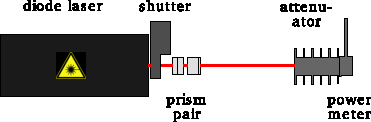
\includegraphics{fig-1}
    \caption{%
        Setup for characterizing the diode laser.
        \parencite[Figure~1]{lab-course/doubling/manual}
    }
    \label{fig:fig-1}
\end{figure}

For measuring the power we just dump the whole beam into a power meter. We
measure the power until we reach \SI{20}{\milli\watt}. 
The data is shown in Figure~\ref{fig:diode-normal}.

\begin{figure}
    \centering
    \includegraphics{diode-normal}
    \caption{%
        Laser power against injection current. The error bars are so small that
        they hide behind the markers. Fitted line stems from a linear fit with
        Jackknife error estimation.
    }
    \label{fig:diode-normal}
\end{figure}

Since the power meter become non-linear beyond \SI{20}{\milli\watt} we use an
attenuator in front of it for larger powers. This will take away a certain
fraction of the beam and allow us to measure higher intensities. The attenuator
has to be calibrated first with small beam powers to allow for a comparison. We
turn the current back down to the lasing threshold in order to get some overlap
between normal and damped laser powers. Then we measure up to
\SI{280}{\milli\ampere} injection current. Our data is shown in
Figure~\ref{fig:diode-both}. In that scale one cannot really see anything
useful, though.

\begin{figure}
    \centering
    \begin{subfigure}[c]{0.48\linewidth}
    \centering
    \includegraphics{diode-both}
    \caption{%
        Linear
    }
    \end{subfigure}
    \hfill
    \begin{subfigure}[c]{0.48\linewidth}
    \centering
    \includegraphics{diode-both-log}
    \caption{%
        Logarithmic
    }
    \end{subfigure}
    \caption{%
        Power ratios with and without attenuator.
    }
\end{figure}

\begin{figure}
    \centering
    \includegraphics{diode-ratio}
    \caption{%
        Calibration of the screw-on attenuator.
    }
    \label{fig:diode-ratio}
\end{figure}

We have checked the background effects and they are negligible. Completely
closing the window did not alter the power readings. Therefore we do not need
to subtract a background value.

The telling quantity is the ratio in the overlap region. As we have not
measured at exactly the same injection currents we need to interpolate the
values. For this we have chosen linear interpolation between the power values
measured as the relation seems linear in Figure~\ref{fig:diode-normal}. Then we
divide the interpolated power values for a given current and obtain a
distinction ratio. Error estimation is performed by resampling our measured
data. For each resampling step we perform the interpolation and build the
ratios. Taking mean and standard deviation for each current value gives the
extinction ratio and error. This is shown in Figure~\ref{fig:diode-ratio}. One
can see that the extinction ratio is in the order of 1000. We will assume that
it is constant for all currents---as the large error band should permit---and
obtain an extinction ratio of $F = \num{<< extinction >>}$.

\subsection{Threshold current}

In Figure~\ref{fig:diode-normal} we have already inserted the linear fit to the
points behind the lasing threshold. We extend the fitted line to the $P = 0$
axis and look for the threshold current~$I_\text{thr}$. We obtain $I_\text{thr}
= \SI{<< threshold >>}{\ampere}$.

Error estimation is performed with the Jackknife method. We perform the fit
four times and leave one of the data points out each time. This way we get a
good error estimate caused by the residuals of the data. From the parameters of
the linear fit the $P = 0$ intersection is computed. Averaging and taking the
standard deviation of the values gives the result. We decided against
resampling as the error bars are way smaller than the residuals, the fit has a
very large $\chi^2$ and renders resampling pointless.

\subsection{Quantum efficiency}

The differential efficiency of the laser is \SI{<< differential_efficiency
>>}{\watt\per\ampere}. This is just the slope~$a$ of the linear fit shown in
Figure~\ref{fig:diode-normal}.

The differential quantum efficiency is the number of photons created per charge
carrier passing the $p$-$n$-junction in the semiconductor
\parencite{fonstad/laser_diodes_1}. In your case we have
\[
    \eta
    = \frac{P/\hbar\omega}{I / e}
    = \frac{P}{I} \frac{e}{\hbar\omega}
    = a \frac{e}{\hbar\omega}
    = \num{<< quantum_efficiency >>} \,.
\]

\subsection{Variable attenuator}
\label{sec:variable_attenuator}

The laser might experience \emph{mode hops} when we adjust the current.
Therefore we do not want to adjust laser power by the current during our
adjustment. We rather want to have an optical way to adjust the beam power. For
this we will use a polarizing beam splitter and a $\lambda/2$-plate in front of
that. By adjusting the polarization of the beam going into the polarizing
splitter we can select the portion of the power advancing to the next parts in
our setup. We extend out setup with a plate and splitter like shown in
Figure~\ref{fig:fig-2}.

\begin{figure}
    \centering
    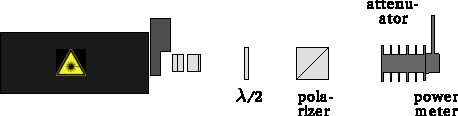
\includegraphics{fig-2}
    \caption{%
        Setup for calibration of the variable attenuator. The laser intensity
        reaching the power meter can be reduces by changing the polarizing with
        a retarder plate. \parencite[Figure~2]{lab-course/doubling/manual}
    }
    \label{fig:fig-2}
\end{figure}

We must obtain a relation of retarder plate angle and output power to use this
later on. There is only one power meter and we want to measure the powers of
both the fundamental and harmonic beam at the same time. We take power
measurements of the fundamental beam in \SI{2.5}{\degree} steps of the retarder
plate.

Our data is shown in Figure~\ref{fig:variable}.
We expect to see a $a \cos(2[\phi - \phi_0])^2 + b$ profile. Our fit parameters
are $\phi_0 = \SI{<< variable_angle_offset >>}{\degree}$, $a = \SI{<<
variable_a >>}{\watt}$ and $b = \SI{<< variable_b >>}{\watt}$.

\begin{figure}
    \centering
    \includegraphics{variable}
    \caption{%
        Measured power with the variable attenuator. Fit is a $a \cos(2[\phi -
        \phi_0])^2 + b$ function.
    }
    \label{fig:variable}
\end{figure}

From this we obtain the extinction ratio $R = (a + b) / b = \num{<<
extinction_ratio >>}$. The large error arises from the very small offset $b$.

\section{Harmonic power}

Now we have the power measurement calibrated. We can determine the power in the
fundamental beam from the angle of the retarder plate. Our setup is extended
with the non-linear crystal and a filter as shown in Figure~\ref{fig:fig-4}.
The blue filter is needed to get rid of the fundamental wave, we only want to
measure the power of the harmonic wave here.

\begin{figure}
    \centering
    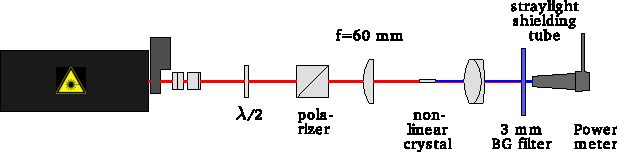
\includegraphics{fig-4}
    \caption{%
        Setup for harmonic power measurement.
        \parencite[Figure~4]{lab-course/doubling/manual}
    }
    \label{fig:fig-4}
\end{figure}

The crystal used here is a $\mathrm{KNbO_3}$ crystal. It has a cross section of
\SI{2}{\milli\meter} times \SI{1.8}{\milli\meter}. It is cut along the b-axis
and has a length of \SI{5}{\milli\meter}. The end faces are coated to avoid
reflections at \SI{987}{\nano\meter} and \SI{494}{\nano\meter}.
\parencite[6]{lab-course/doubling/manual}

\subsection{Output power optimization}

With the rough optical setup in place we can insert the crystal and optimize
for maximum harmonic power. We slowly heat up the crystal to \SI{36}{\celsius}.
Then we slide it into the focus of our setup. It took a bit to adjust this. One
important thing to keep in mind is that the crystal is very small. Therefore
one needs to move the crystal through the beam and identify the edges of the
crystal in the beam.

The blue harmonic light is focused with an achromatic lens and filtered with an
\SI{3}{\milli\meter} BG40 glass filter. From Figure~3 from
\parencite{lab-course/doubling/manual} we estimate a total transmission
coefficient of \num{0.9} at \SI{494}{\nano\meter}. For the unwanted fundamental
wave we have a transmission coefficient of around $10^{-2.3} = 0.005$.

The maximum laser power is in the order of magnitude \SI{150}{\milli\watt}. We
know this from the measurement with the attenuator (data in
Section~\ref{sec:variable_attenuator_table}) and the suppression ratio of
around a thousand. The BG40 filter will only let $1/200$ of that through,
therefore we have less than one milliwatt of fundamental wave behind the filter
plate. This is still more than the fundamental power. Therefore we hope that
the power meter has a sufficient filtering on its own.

After doing this we were able to measure some \SI{40}{\micro\watt} of blue
light. Once the power meter is set up again we tune all the parameters a bit to
optimize this power. This also includes the rotation of the polarizing beam
splitter. Unfortunately we did not record the original position from the
calibration measurement and now have an offset angle in the relation between
the $\lambda/2$-plate angle and the laser power from the variable attenuator.
This is something that we can recover from later on, though.

\subsubsection{Beam waist and Rayleigh length}

We know that the focal length of the used lens is $f = \SI{60}{\milli\meter}$.
Since the incoming laser beam is collimated, we know that the distance $z$
between the focus and the lens is just this $f$. The diameter of the collimated
beam is given by $w(z) = \SI{3.5 +- 0.5}{\milli\meter}$
\parencite[8]{lab-course/doubling/manual}.

One can let Mathematica solve the relations describing the beam waist to give
an expression for the Rayleigh length $z_0$:
\[
    z_0 = \piup \frac{n w(z)^2 \pm \sqrt{n^2 w(z)^4 - 4 \lambda_0^2 z^2}}{2 \lambda_0} \,.
\]
The problem here is that we do know which branch of the solution to take. One
will give a very small Rayleigh length, the other one tens of meters. There is
another way to go about this. We first compute the asymptotic beam angle
\[
    \theta = \arctan\del{\frac{w(z)}{z}} = \SI{<< theta >>}{\radian} \,.
\]
Then we compute the waist
\[
    w_0 = \frac{\lambda}{\piup \theta} = \SI{<< waist_mum >>}{\micro\meter} \,.
\]
From here we obtain the Rayleigh length
\[
    z_0 = \frac{n \piup w_0^2}{\lambda}
    = \SI{<< rayleigh_length_mm >>}{\milli\meter} \,.
\]
The errors are so large because the uncertainty in the beam diameter is very
large.

The normalized crystal length is $\xi = l/b = \num{<< normalized_length
>>}$.
For the optimal case we would need to have $\xi_0 = \num{2.84}$. Given the large
error margin our result $\xi$ could be close enough to $\xi_0$. The more
accurate approach is to perform a one-sample $t$-test. Our null hypothesis is
$\xi = \xi_0$. Can we disprove the null hypothesis, i.e.\ is there no
measurable deviation given the large error of the beam diameter? The test
statistic is $T = \num{<< boyd_kleinman_ttest_t >>}$. Intuitively one can think
of this as the distance of $\xi$ to $\xi_0$ in terms of the standard error
(standard deviation reduced by $\sqrt N$, $N = 1$ is the sample count here).
A look into a table with percentiles of the $t$-distribution tells us that for
a two-sided test with a confidence level of $\alpha = 0.6$ the $|T|$ would have
to be greater than 1.376 for us to reject the null hypothesis
\parencite{wikipedia/student_t}. If we want a higher rejection power, we would
set $\alpha = 0.05$ but would incur a quantile value of 12.71 which $|T|$ would
have to exceed for us to reject the null hypotheses. Therefore we must accept
the null hypothesis and say that the Boyd-Kleinman condition is fulfilled.

The optimal focal length can be derived as follows: We want $l/b = \xi_0 =
2.84$. Therefore we need $z_0 = l/(2\xi_0)$ and
\[
    w_0^2 = \frac{l \lambda_0}{2n\piup\xi_0} \,.
\]
Using the relation for the beam radius we can derive
\[
    z^2 = \sbr{
        \frac{2n \piup w(z)^2 \xi_0}{l \lambda_0} - 1
    } \frac{l^2}{4 \xi_0^2} \,.
\]
Plugging in the numbers we obtain an optimal $f = z$ of \SI{<<
optimal_focal_length_mm >>}{\milli\meter}.

\subsection{Crystal temperature dependence}

Since the index of refraction is temperature depending on our crystal material
we want to measure the temperature dependence. First we cool down to
\SI{27}{\celsius} in steps of \SI{0.5}{\celsius} (to protect the crystal) and
then heat up to \SI{40}{\celsius} in steps of \SI{0.2}{\celsius}. While heating
up take measurements of the harmonic power.

Our measurements are shown in Figure~\ref{fig:temperature}. We fit a $\sinc$
function with
\[
    P(T) = a \sinc\del{\frac{T - c}{b}} + d \,.
\]
The fit parameters are
\[
    a = \SI{<< temp_amplitude >>}{\watt}
    \,,\quad
    b = \SI{<< temp_width >>}{\celsius}
    \,,\quad
    c = \SI{<< temp_center >>}{\celsius}
    \,,\quad
    d = \SI{<< temp_offset >>}{\watt} \,.
\]
Error estimation is done via resampling.

\begin{figure}
    \centering
    \includegraphics{temperature}
    \caption{%
        Temperature dependence of the harmonic power. Fitted is a $\sinc$
        function. Error estimation is done via resampling.
    }
    \label{fig:temperature}
\end{figure}

The fit clearly has a very high $\chi^2$, the sinc-model does not describe the
data well. Also the shape is not symmetric. This is actually not a surprise,
a symmetric shape would be one. There should be a sinc-shape with respect to
the phase difference $\Deltaup k$. By changing the temperature we change the
refractive indices of the axes to get a better match for $n_\omega$ and
$n_{2\omega}$. The dependence $n(T)$ must not be linear, it can have a more
complicated structure. Also the dependence of $\Delta k$ on both refractive
indices has to be taken into account. Therefore it is no surprise that the
shape $P(T)$ is not symmetric.

Now that we know the optimal temperature for the crystal, we slowly tune the
temperature to this optimal setting.

\subsection{Input power dependence}

The output power must depend on the input power. As we have calibrated in
Section~\ref{sec:variable_attenuator}, we should be able to choose an input
power by rotating the retarder plate in front of the splitter. As we have
rotated the polarizing beam splitter without thinking about this step, we will
need to adjust for the offset angle after this measurement. Then we can shift
the first measurement and have the desired angle--power relation. We hope that
there is no fundamental offset that we would miss this way. There is no
physical reason to have such an offset, we should be just fine.

We measure the output power while adjusting the angle of the retarder plate.
Our data is shown in Figure~\ref{fig:harmonic-splitter}. As the harmonic
intensity should scale with the square of the fundamental intensity we expect a 
\[
    P'(\phi) = a' \cos(2 [\phi - \phi_0'])^4 + b'
\]
relationship here. The fit parameters are
\[
    \phi_0' = \SI{<< splitter_angle_offset >>}{\degree}
    \,,\quad
    a' = \SI{<< splitter_a >>}{\watt}
    \,,\quad
    b' = \SI{<< splitter_b >>}{\watt} \,.
\]
Error estimation is done via resampling. We can see that the offset angle has
changed just a little bit. Just what we have expected since we turned the
polarizing beam splitter a little bit. The model seems to fit the data rather
well, there are slight deviations, especially at the left peak.

We have measured from large angles to small angles. At \SI{75}{\degree} we
encountered large deviations, the data points prior (larger angle) also show
larger fluctuations than the previous points. Perhaps we have noticed the
fluctuations too late and should have increased the error estimation for the
points around \SI{90}{\degree} as well. The right peak does not show this
pattern of deviation. Therefore we do not think that there is saturation in any
of the components.

\begin{figure}
    \centering
    \includegraphics{harmonic-splitter}
    \caption{%
        Harmonic power depending on the $\lambda/2$-plate angle. Fitted is a
        $\cos(2\phi)^4$ function. Error estimation via resampling.
    }
    \label{fig:harmonic-splitter}
\end{figure}

Using the amplitudes $a$ and $a'$ of the fit functions to the angular power
distribution of fundamental and harmonic wave, respectively, we can obtain the
power ratio. The amplitude of the harmonic wave has to be corrected by the
screw-on attenuator factor $F$. We therefore have the power ratio
\[
    \eta' = \frac{P_\text{har}}{P_\text{fun}} = \frac{a'}{a F}
    = \num{<< efficiency >>} \,.
\]
In the manual the definition is
\[
    \eta = \frac{P_\text{har}}{P_\text{fun}^2}
    = \frac{a'}{[a F]^2}
    = \SI{<< efficiency_sq >>}{\per\watt} \,.
\]
This does not seem to make much sense as an efficiency due to the unit. An
efficiency should be dimensionless. By using the fit parameters $a$ and $a'$ we
dodged the problem with the angle offset that we mentioned earlier. We
basically assume that the angular distributions align perfectly and then we
can just take the fit parameters. The offsets $b$ and $b'$ are neglected here
as they are so small.

\subsection{Input polarization dependence}

By taking out the polarizing beam splitter we can freely adjust the linear
polarization of the light that goes into the crystal. We take a set of
measurements of the output power with different angles of the retarder plate.
Our data is shown in Figure~\ref{fig:harmonic-bare}.

\begin{figure}
    \centering
    \includegraphics{harmonic-bare}
    \caption{%
        %
    }
    \label{fig:harmonic-bare}
\end{figure}

As we use temperature phase matching we expect to only have a type 1 phase
matching there. Hence the output power should just depend on one component of
the polarization. As the output power scales quadratically with the input
power, we expect a quartic cosine again. We fit the same function as above and
obtain
\[
    \phi_0' = \SI{<< bare_angle_offset >>}{\degree}
    \,,\quad
    a' = \SI{<< bare_a >>}{\watt}
    \,,\quad
    b' = \SI{<< bare_b >>}{\watt}
\]
this time. The offset angle has changed a little bit. This would be explained
if the polarizing beam splitter has not been perfectly aligned previously.
Since only type 1 phase matching works with this crystal, the incident light
should be polarized parallel to one of the crystal axes. The polarizing beam
splitter has been close to parallel to the crystal but apparently still off by
say \SI{1.5}{\degree}. The maximum power has gone up slightly, this is probably
due to the losses in the beam splitter. Then the background has tripled but is
still rather small. This could be slightly changed light conditions (window
opened a little bit more) and lack of extinction from the beam splitter at
crossed polarization.

\section{Wavelength comparison}

As this experiment is titled \emph{frequency doubling} we except that the
frequency of the incident beam has doubled pretty much exactly. In the
following parts we will compare the two wavelengths with each other and
determine how exact the doubling actually is.

\subsection{Grating}

The first and quick method is using a grating to have a wavelength dependent
diffraction. As the diffraction angle scales with diffraction order $n$ and
wavelength $\lambda$ as a quotient we would expect to see an overlap of the
$n$-th order fundamental wave and the $2n$-th order harmonic wave.

We take photographs of the of the laser spots on the wall. Starting with the
zeroth order, we take a picture without the IR-card, our CCD-camera should only
be pick up the harmonic wave. Then we hold the IR-card against the wall and see
a bright green spot. We take a picture of that fundamental wave as well. In
Figure~\ref{fig:grating-2} both pictures are shown together with the difference
of the images. In the zeroth order the beams must coincide trivially and indeed
we see a rotationally symmetric difference image. As far as we can tell the
beams overlap.

Then we advance to the next order. We expect to see only harmonic light there,
no fundamental wave. When we hold the IR-card over the blue spot, no green
light appears. Our images are shown in Figure~\ref{fig:grating-4}. This tells
us that the harmonic frequency is larger than the fundamental one, just as we
expect. Going to the next spot on the wall we do the same procedure again. Now
we do see a bright green with the IR-card. See Figure~\ref{fig:grating-1} for
the triplet of images.

\begin{figure}[p]
    \centering
    \begin{subfigure}[c]{0.3\linewidth}
        \centering
        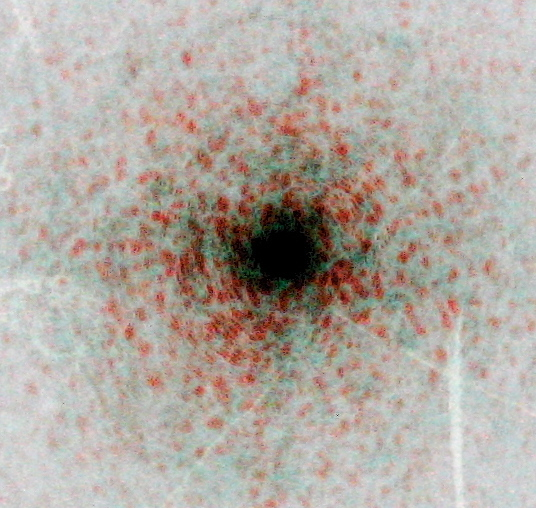
\includegraphics[width=\linewidth]{grating-2-crop-blue}
        \caption{%
            harmonic
            }
    \end{subfigure}
    \hfill
    \begin{subfigure}[c]{0.3\linewidth}
        \centering
        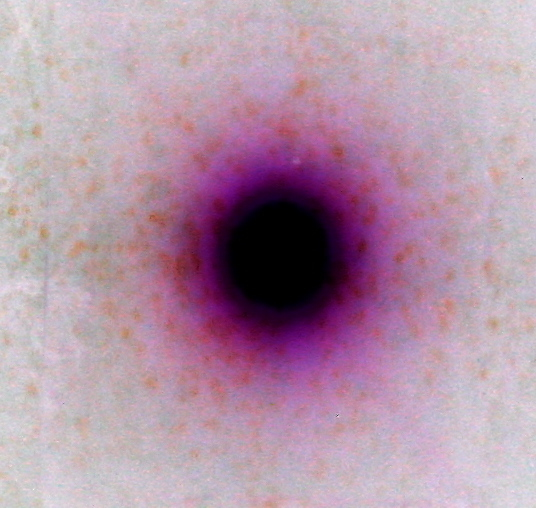
\includegraphics[width=\linewidth]{grating-2-crop-red}
        \caption{%
            fundamental
            }
    \end{subfigure}
    \hfill
    \begin{subfigure}[c]{0.3\linewidth}
        \centering
        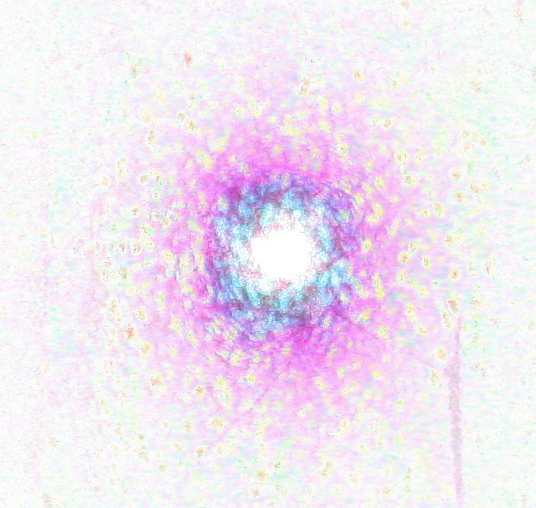
\includegraphics[width=\linewidth]{grating-2-crop-diff}
        \caption{%
            difference
            }
    \end{subfigure}
    \caption{%
        Zeroth order of both beams. As the difference is rotationally
        symmetric, both beams coincide. Trivial for zeroth order.
        }
    \label{fig:grating-2}
\end{figure}

\begin{figure}[p]
    \centering
    \begin{subfigure}[c]{0.3\linewidth}
        \centering
        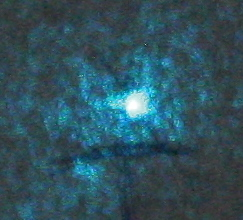
\includegraphics[width=\linewidth]{grating-4-crop-blue}
        \caption{%
            harmonic
            }
    \end{subfigure}
    \hfill
    \begin{subfigure}[c]{0.3\linewidth}
        \centering
        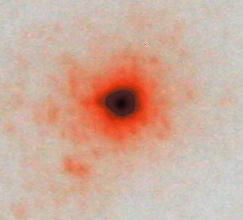
\includegraphics[width=\linewidth]{grating-4-crop-red}
        \caption{%
            fundamental
            }
    \end{subfigure}
    \hfill
    \begin{subfigure}[c]{0.3\linewidth}
        \centering
        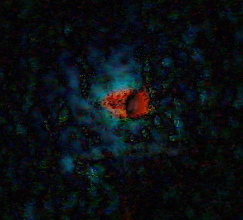
\includegraphics[width=\linewidth]{grating-4-crop-diff}
        \caption{%
            difference
            }
    \end{subfigure}
    \caption{%
        First order harmonic. There is no fundamental wave scattered in this
        angle.
        }
    \label{fig:grating-4}
\end{figure}

\begin{figure}[p]
    \centering
    \begin{subfigure}[c]{0.3\linewidth}
        \centering
        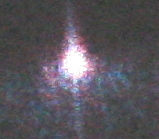
\includegraphics[width=\linewidth]{grating-1-crop-blue}
        \caption{%
            harmonic
            }
    \end{subfigure}
    \hfill
    \begin{subfigure}[c]{0.3\linewidth}
        \centering
        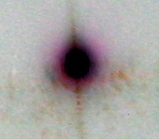
\includegraphics[width=\linewidth]{grating-1-crop-red}
        \caption{%
            fundamental
            }
    \end{subfigure}
    \hfill
    \begin{subfigure}[c]{0.3\linewidth}
        \centering
        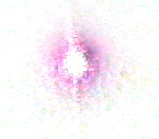
\includegraphics[width=\linewidth]{grating-1-crop-diff}
        \caption{%
            difference
            }
    \end{subfigure}
    \caption{%
        Second spot. This is the first fundamental and the second harmonic
        maximum. As the difference is rotationally symmetric, both beams
        coincide, frequencies must be simple multiples.
        }
    \label{fig:grating-1}
\end{figure}

As we see a fundamental wave scattered here we can conclude that the frequency
is indeed doubled. Since all the spots coincide perfectly to the available
precision we cannot rule out a perfect doubling of the frequency here.

We should have exchanged the collimating lens to the one with
\SI{125}{\milli\meter}. Unfortunately we just used the \SI{30}{\milli\meter}
lens. Therefore the beam diameter is a factor \num{4.17} smaller than it
should. The number of slits illuminated on the grating is therefore reduced by
this number as well. This is not too bad as we will perform a way more accurate
measurement next anyway.

The beam coming from the laser has a diameter of \SI{3.5(5)}{\milli\meter}.
Our lens configuration acts like a telescope and halves the diameter. The
line count on the grating is \SI{600}{\per\milli\meter}. The number of lines
illuminated is therefore \num{<< illuminated >>}. Using the equation $\Deltaup
\lambda / \lambda = nN$ from the theory section we can conclude that we have a
relative theoretical error of \num{<< rel_error >>}.

We did not measure the distances used carefully, therefore we cannot produce a
sketch here. However, we can give an order of magnitude estimation for the
resolution obtained. We used the grating to project the beams onto the wall of
the room. The distance was around \SI{1.5}{\meter}. Let's assume we could see
if the fundamental and harmonic beams had a separation of \SI{1}{\milli\meter}.
Using the CCD camera subtraction images we might achieve higher resolutions but
the camera was not part of the official setup. Then by the relation between
angle $\phi_n$ and wavelength $\lambda$, Equation~\eqref{eq:phi_grating}, we
can infer with Gaussian error propagation that $\Deltaup \lambda / \lambda =
\cos(\phi_n) \Deltaup \phi / \phi$. Since we do not know the angle we just
assume $\cos(\phi_n) = 1$ and potentially undererstimate the resolution. Using
those numbers we obtain
\[
    \frac{\Deltaup \lambda}{\lambda} = \num{6.7e-4} \,.
\]
This is better than the theoretical resolution. We have assumed that we can
distinguish \SI{1}{\milli\meter} of separation by looking at it. We can do this
in our case as we can toggle both peaks individually by using the IR-card. If
that was not the case and they would have the same color to the eye, then one
would need a clear separation of the peaks. The closest that we could separate
two intense green beams would be larger then \SI{4}{\milli\meter}. Then we
would be clearly worse than the theoretical resolution.

\subsection{Michelson interferometer}

The rough confirmation of the frequency doubling can be made more precise with
a Michelson interferometer. The setup which we are going to build now is shown
in Figure~\ref{fig:fig-5}. First we set up the top mirror to reflect the light
onto the moving mirror. Once the blue dot on the moving mirror did not waver
any more, the top mirror is set. Then we insert the glass plate such that
the beams going to the left and right were parallel to the screw holes on the
table. After that we add the right mirror and make sure that the beam coincides
with the one reflected via the bottom mirror.

\begin{figure}
    \centering
    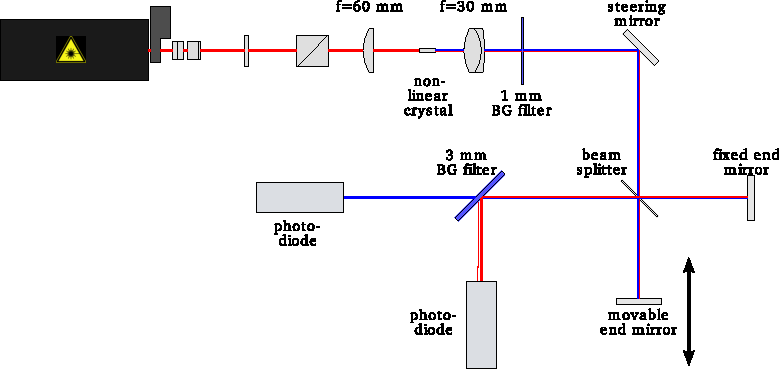
\includegraphics{fig-5}
    \caption{%
        Michelson interferometer setup. The light comes from the laser and
        enters the interferometer from the north. It is then split to east and
        south, reflected back and exits on the west. The thick BG40 filter
        separates the two wavelengths such that we can detect them separately.
        \parencite[Figure~5]{lab-course/doubling/manual}
    }
    \label{fig:fig-5}
\end{figure}

Then we install the thick BG40 filter behind the glass plate. Behind the filter
we have two fast photo diodes. One will receive the light from the fundamental
wave and a negligible part of the harmonic wave. The other one will receive the
harmonic wave and a severely suppressed part of the fundamental wave. We should
be able to take it as a perfect split.

By looking at the photo diode signal versus time we obtained images like the
one shown in Figure~\ref{fig:two-waves-15}. There one can nicely see that the
bottom wavelength is half of the top one. This is not a very precise
measurement, it is more for the intuition. The smearing of the curves in the
right part of the oscillogram stems from the non-constant $\dot d_1$ which
drives this oscillation. Since we push the slide by hand we of course
accelerate it. This smearing rises from $\ddot d_1$ induced. The left side is
sharper since there the signal is freshly triggered.

\begin{figure}
    \centering
    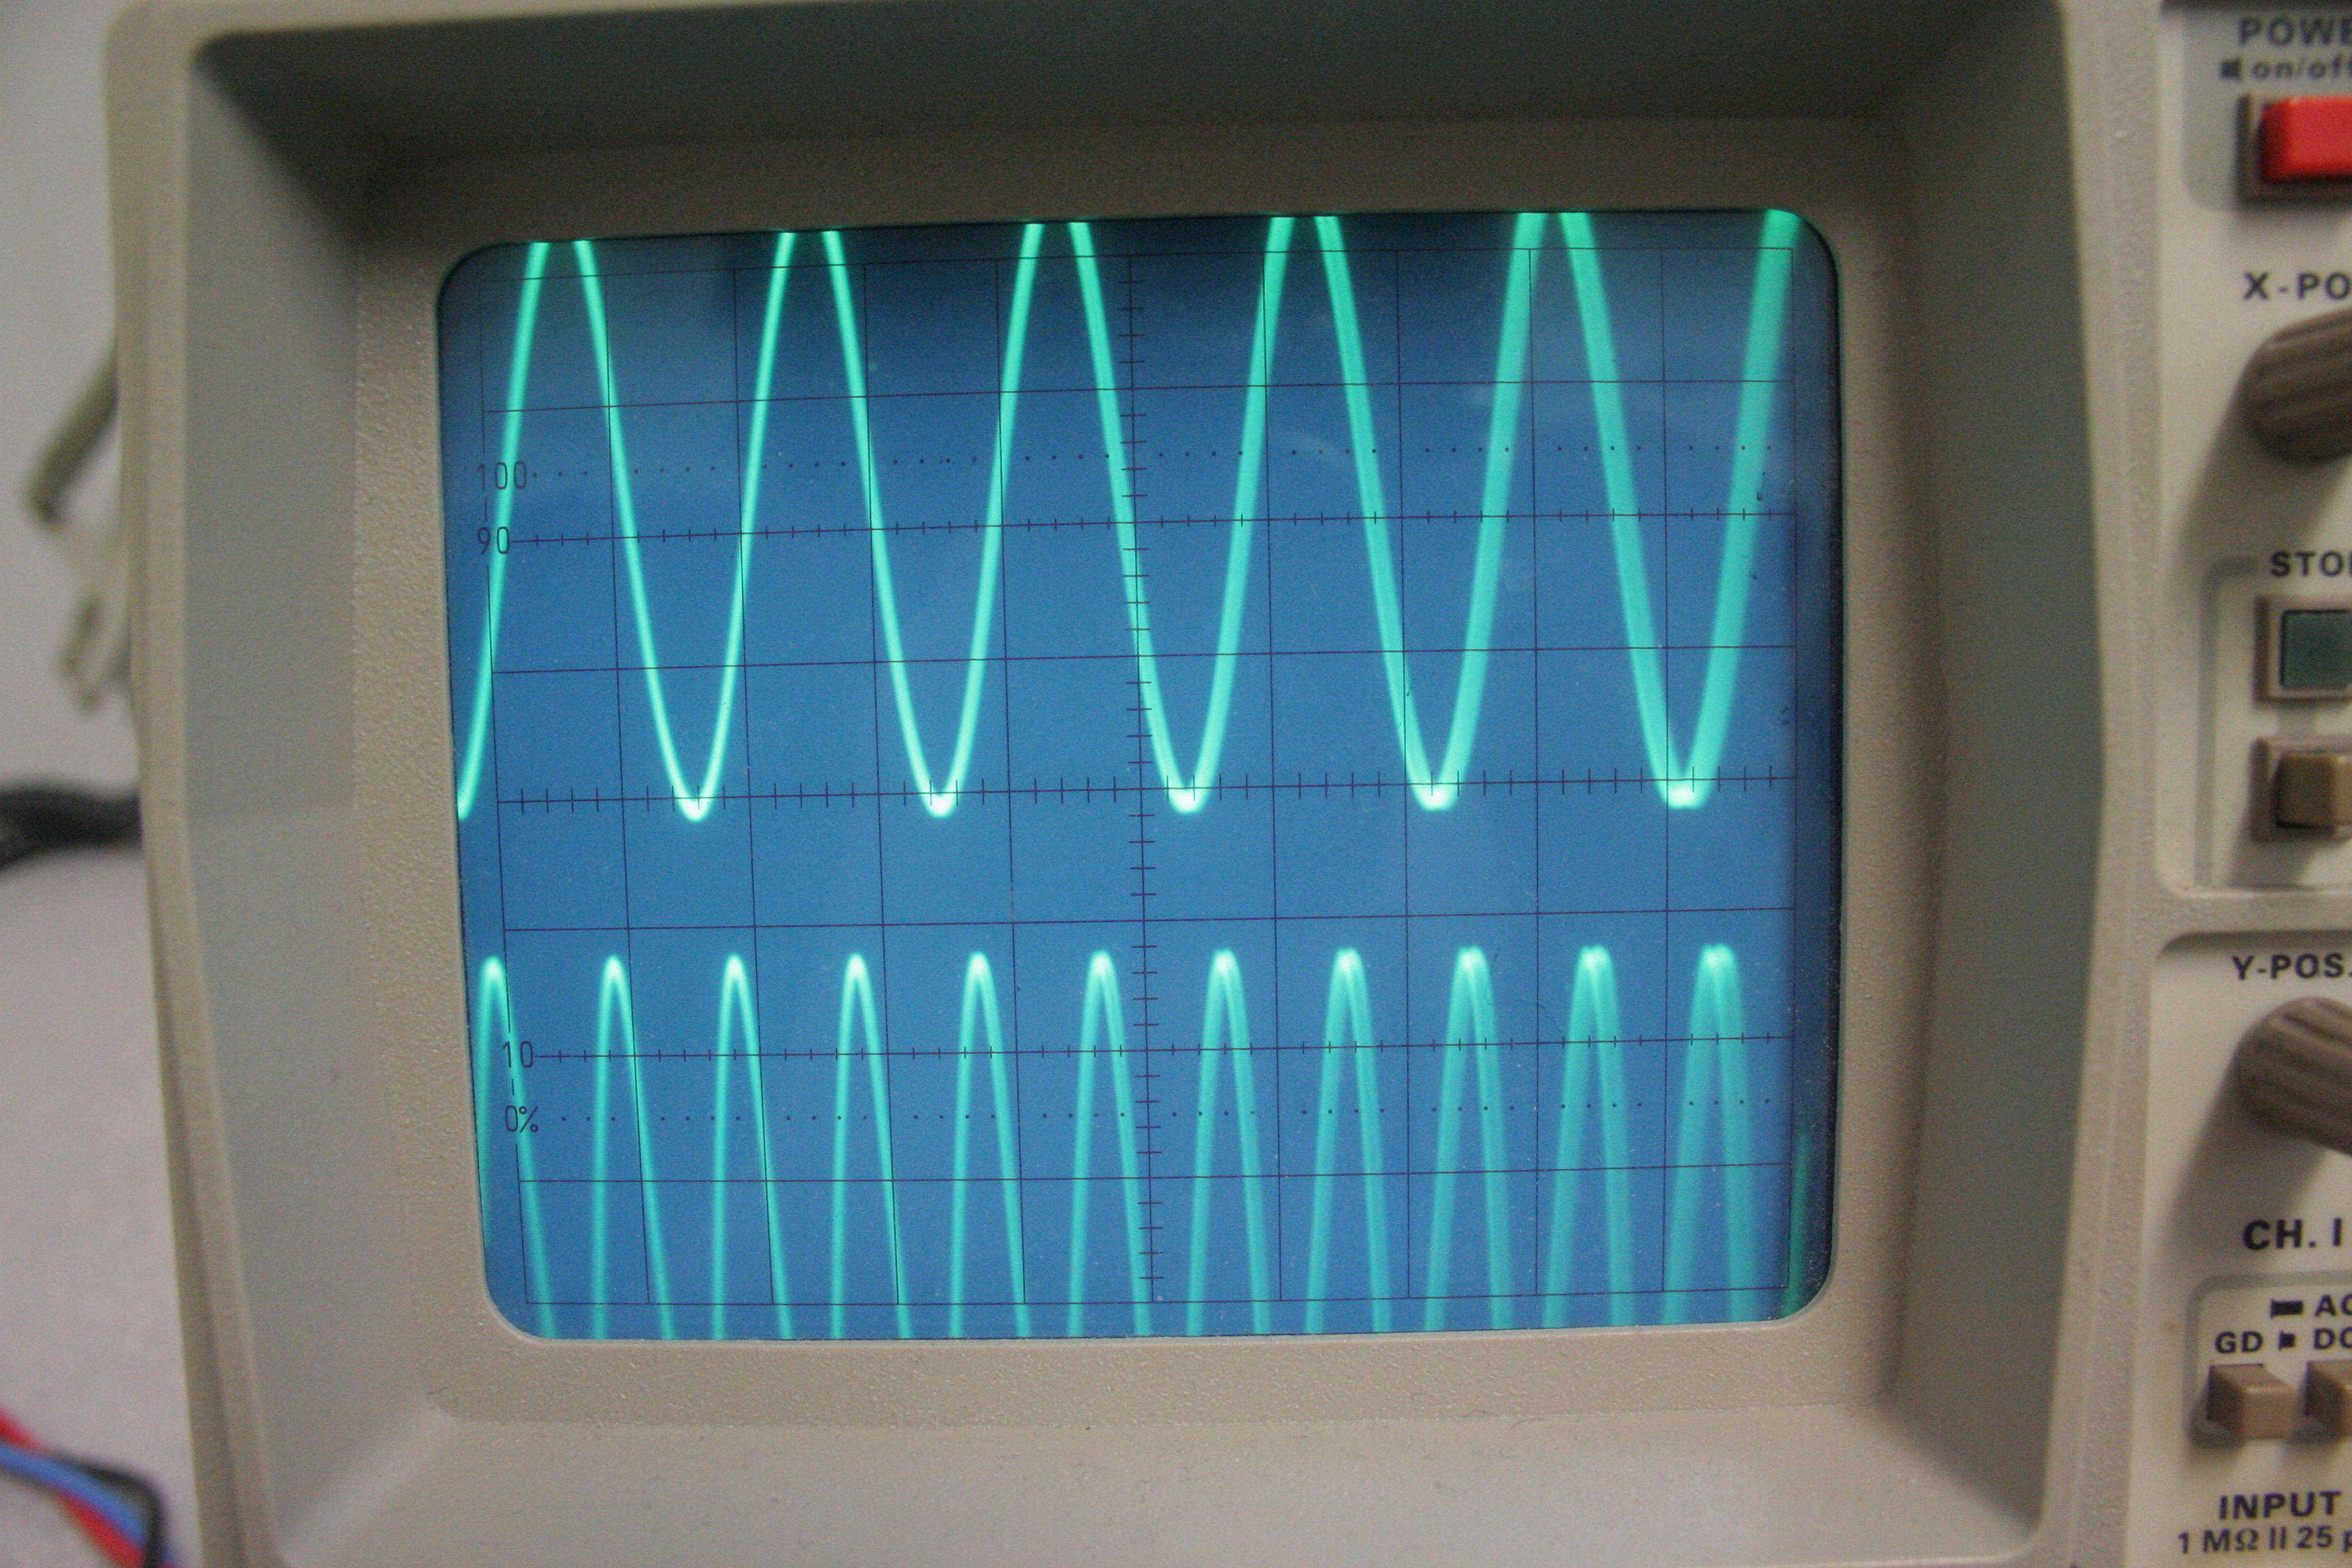
\includegraphics[width=0.8\linewidth]{two-waves-15}
    \caption{%
        Fundamental and harmonic wave signal for comparison. Triggered.
        Desaturated, inverted.
    }
    \label{fig:two-waves-15}
\end{figure}

Hooking both photo diodes to the oscilloscope in $x$-$y$-mode, we obtain some
Lissajous figures as shown in Figure~\ref{fig:lissajous-measured} by slightly
moving the movable mirror. It was sufficient to touch the slide, our bodies
apparently cause enough vibration to move it by nanometers. In
Figure~\ref{fig:lissajous-01} one can see a \enquote{figure 8} Lissajous
figure. It has been rather stable when holding the slide at one position and
just vibrating it. If there was any violation from the $2:1$ ratio, the
Lissajous figure would rotate on its own. We did not observe any of that,
therefore we conclude that the ratio is exact in the realm of the resolution
available. The other image shows the \enquote{U shape} that can only come from
a $2:1$ ratio as well. The broadening of the shapes comes from the nonzero
$\ddot d_1$, we do not think that the frequency ratio is not exact.

\begin{figure}
    \centering
    \begin{subfigure}[c]{0.48\linewidth}
        \centering
        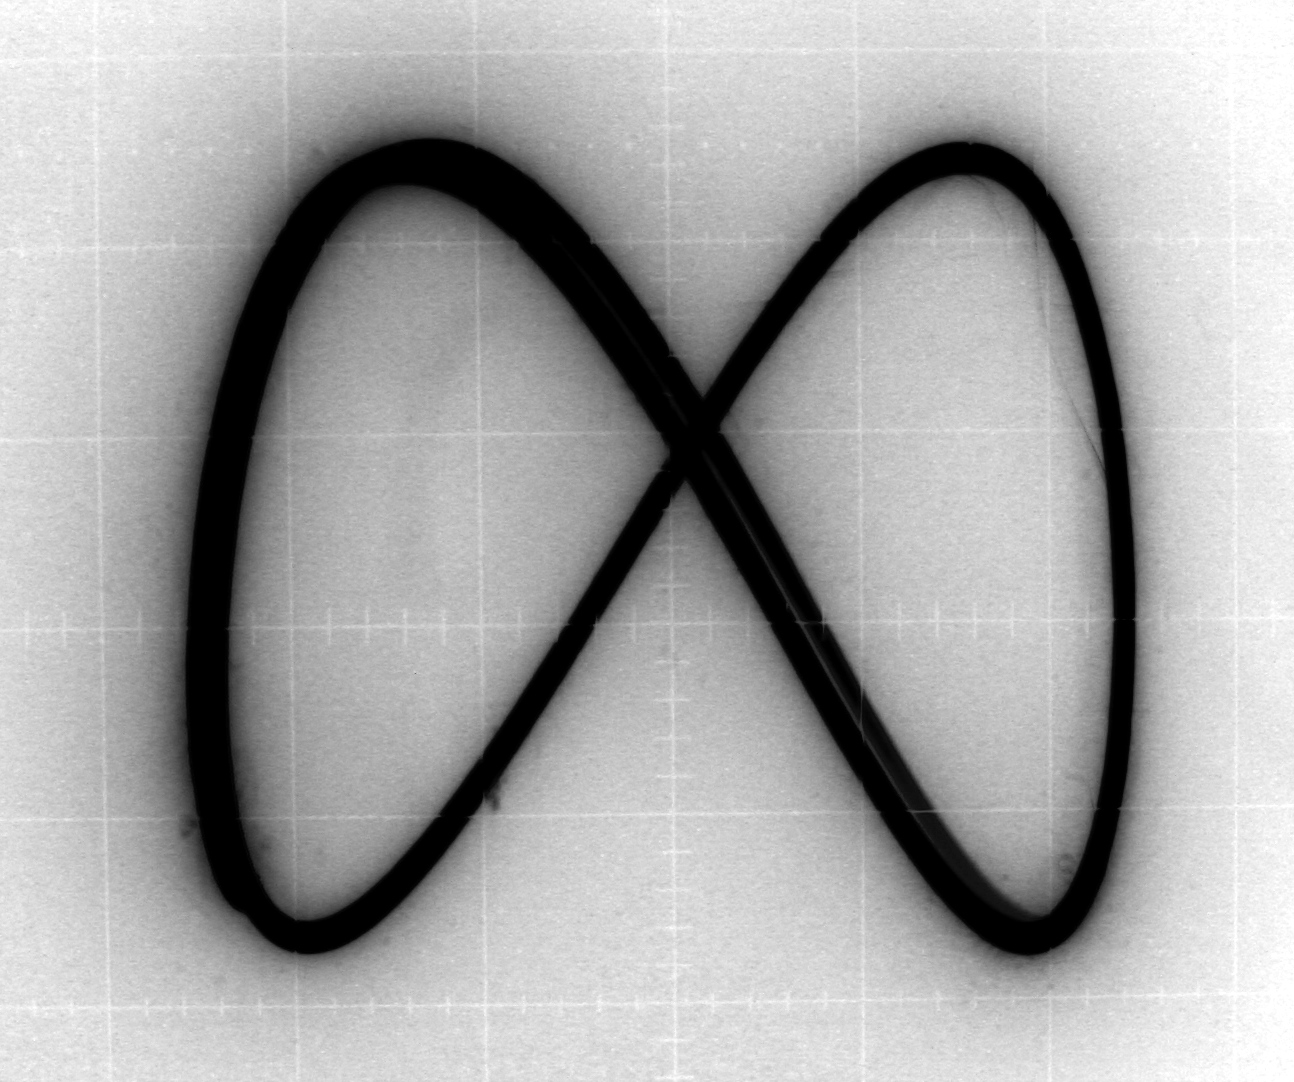
\includegraphics[width=\linewidth]{lissajous-01}
        \caption{%
            %
            }
        \label{fig:lissajous-01}
    \end{subfigure}
    \hfill
    \begin{subfigure}[c]{0.48\linewidth}
        \centering
        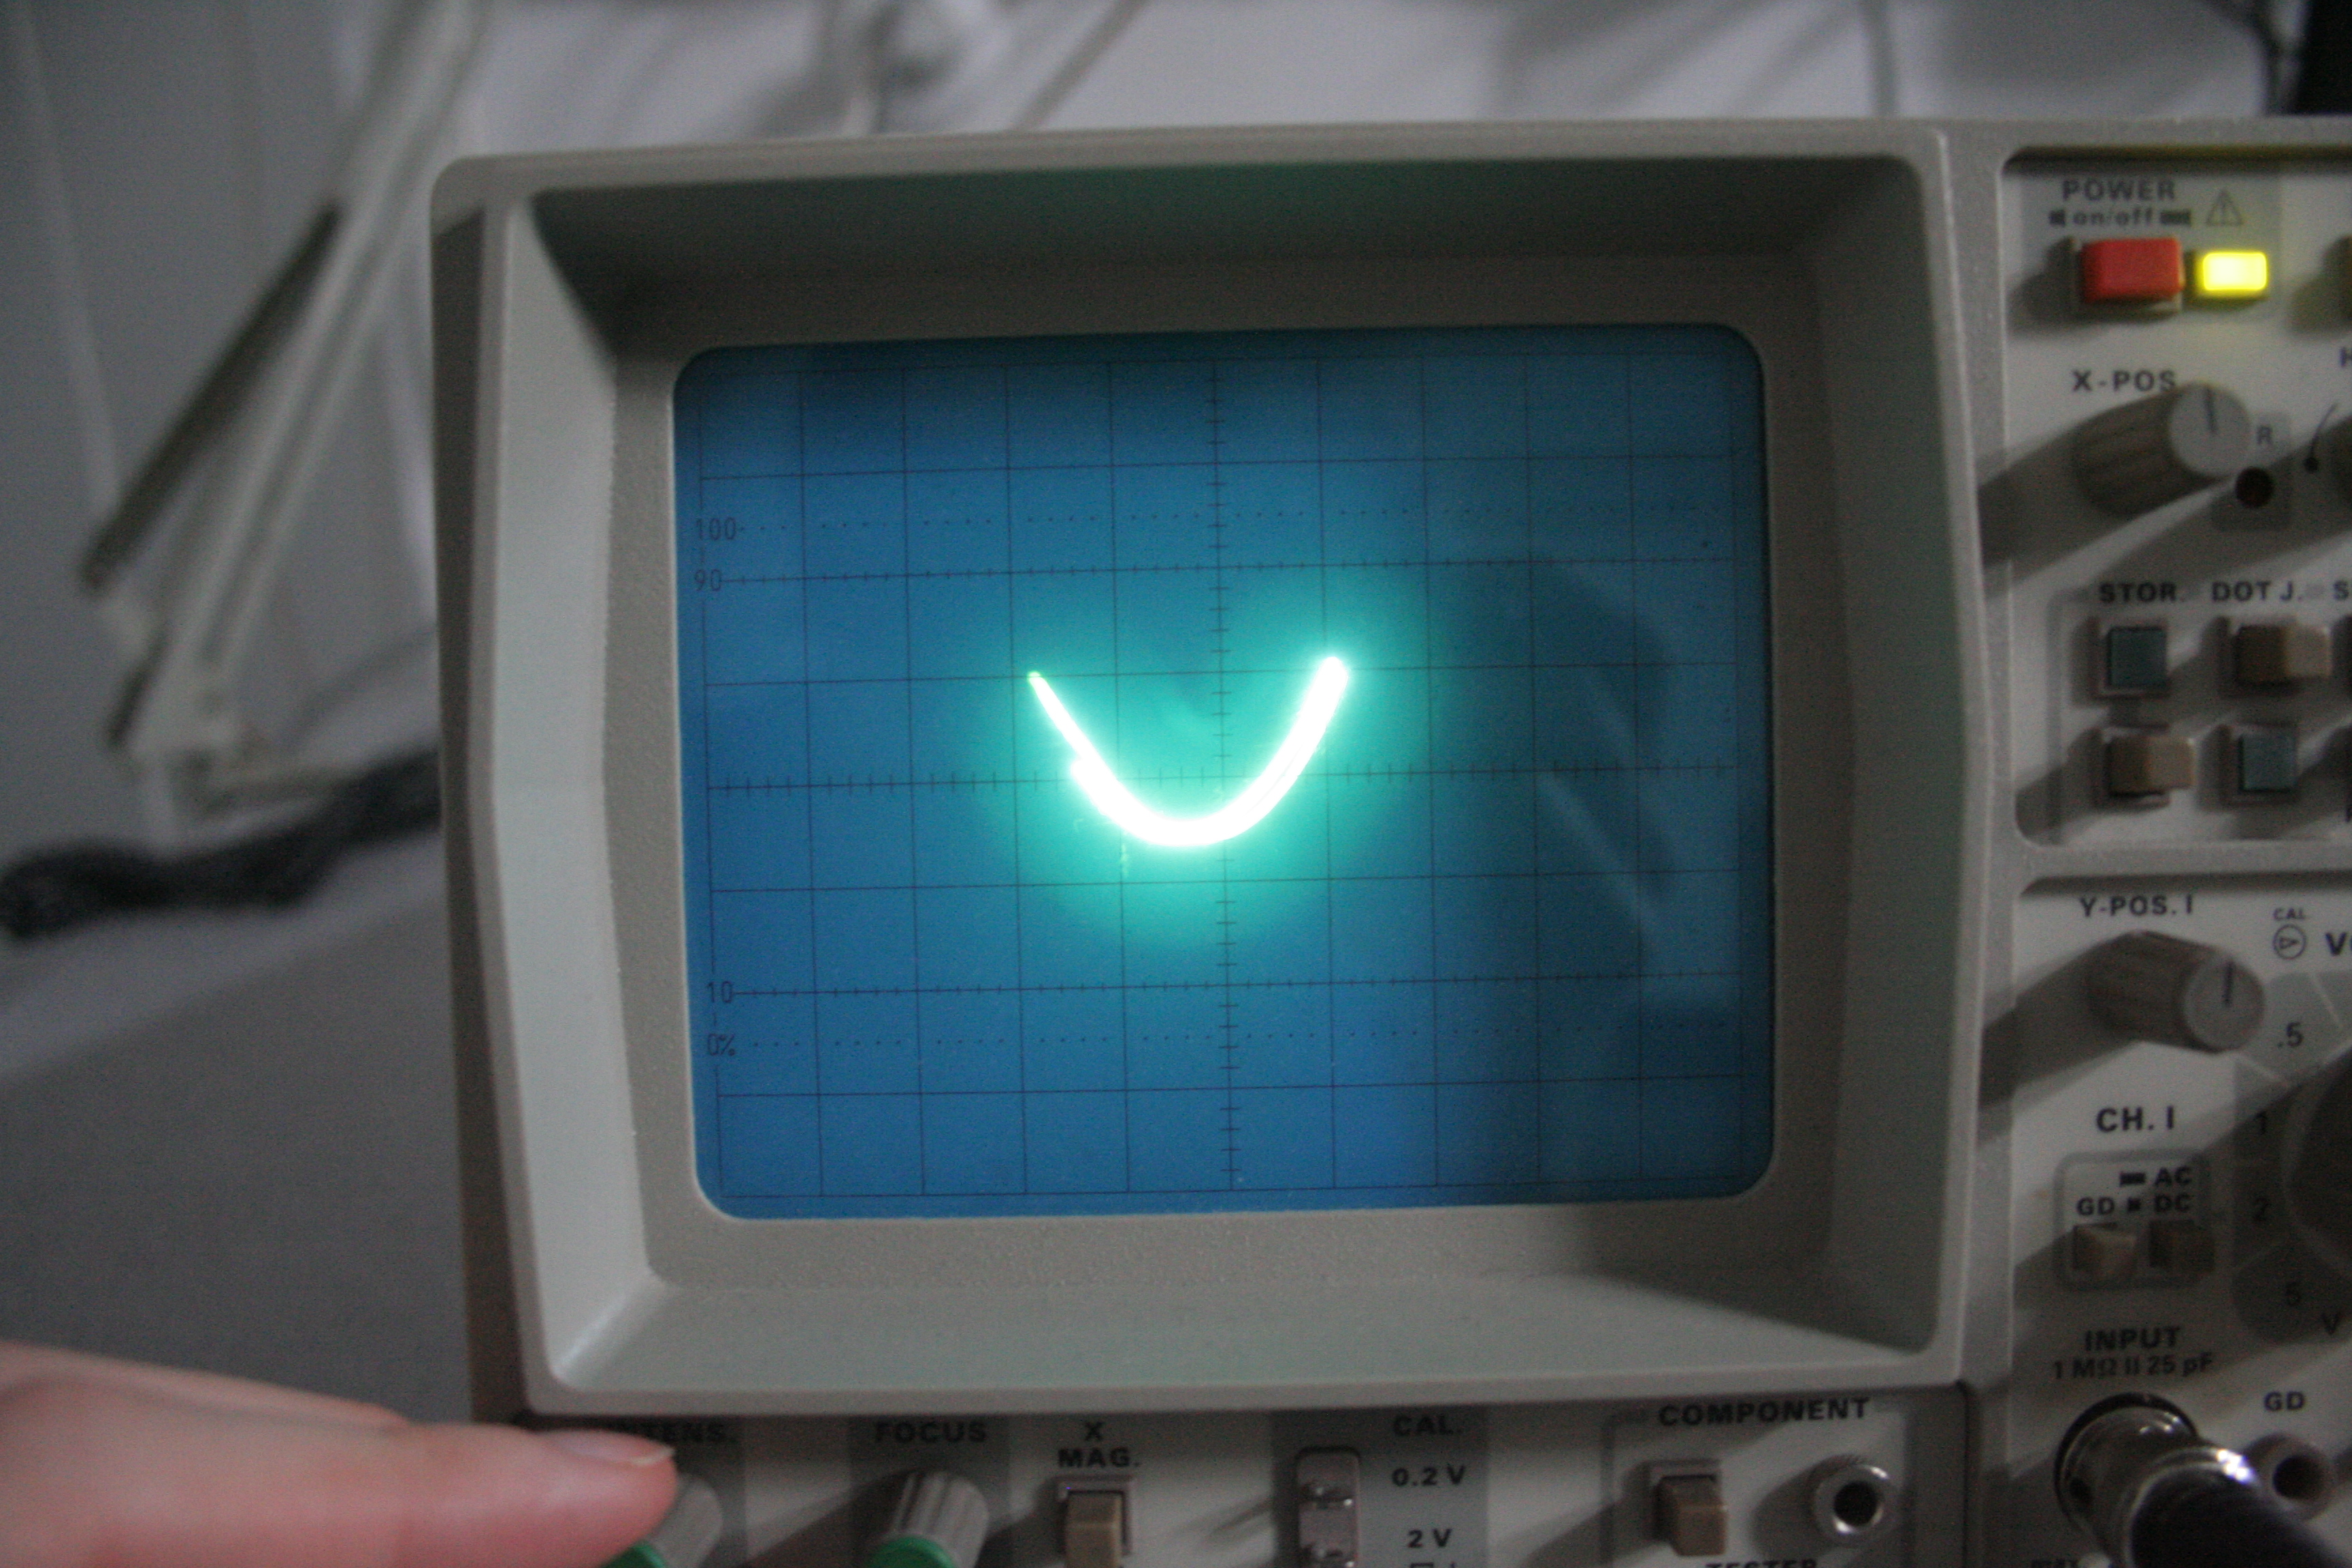
\includegraphics[width=\linewidth]{lissajous-08}
        \caption{%
            %
            }
    \end{subfigure}
    \caption{%
        Observed Lissajous figures. Desaturated, inverted.
        }
    \label{fig:lissajous-measured}
\end{figure}

% TODO (Lino) Compare with literature values.
% TODO (Lino) Compute spectral resolution of the interferometer.

\begin{appendix}
    \chapter{Tables}

    \section{Diode laser power without attenuator}

    \begin{tabular}{SS}
        \toprule
        {$I/\si{\milli\ampere}$}
        & {$P/\si{\nano\watt}$} \\
        \midrule
        %< for row in diode_normal_table >%
        << ' & '.join(row) >> \\
        %< endfor >%
        \bottomrule
    \end{tabular}

    \section{Diode laser power with attenuator}

    \begin{tabular}{SS}
        \toprule
        {$I/\si{\milli\ampere}$}
        & {$P/\si{\nano\watt}$} \\
        \midrule
        %< for row in diode_damped_table >%
        << ' & '.join(row) >> \\
        %< endfor >%
        \bottomrule
    \end{tabular}

    \section{Angle dependence of variable attenuator}
    \label{sec:variable_attenuator_table}

    \begin{longtable}[l]{SS}
        \toprule
        {$\phi/\si{\degree}$}
        & {$P/\si{\nano\watt}$} \\
        \midrule
        \endhead
        %< for row in variable_attenuator_table >%
        << ' & '.join(row) >> \\
        %< endfor >%
        \bottomrule
    \end{longtable}

    \section{Temperature dependence of harmonic power}

    \begin{longtable}[l]{SS}
        \toprule
        {$T/\si{\celsius}$}
        & {$P/\si{\nano\watt}$} \\
        \midrule
        \endhead
        %< for row in temperature_table >%
        << ' & '.join(row) >> \\
        %< endfor >%
        \bottomrule
    \end{longtable}

    \section{Angle dependence with splitter}

    \begin{tabular}{SS}
        \toprule
        {$\phi/\si{\degree}$}
        & {$P/\si{\nano\watt}$} \\
        \midrule
        %< for row in harmonic_splitter_table >%
        << ' & '.join(row) >> \\
        %< endfor >%
        \bottomrule
    \end{tabular}

    \section{Angle dependence without splitter}

    \begin{tabular}{SS}
        \toprule
        {$\phi/\si{\degree}$}
        & {$P/\si{\nano\watt}$} \\
        \midrule
        %< for row in harmonic_bare_table >%
        << ' & '.join(row) >> \\
        %< endfor >%
        \bottomrule
    \end{tabular}

\end{appendix}

\end{document}

% vim: spell spelllang=en_us tw=79
